% ==============================================================================
% CAPÍTULO 5: ANÁLISIS DE SENSIBILIDAD Y TOLERANCIA DE RADIOFRECUENCIA
% ==============================================================================
\chapter{Análisis de Sensibilidad y Tolerancia de Radiofrecuencia}

\section{Modelo Teórico de Descalce de Frecuencia y Desplazamiento Síncrono}
En la operación real de una cavidad resonante tipo Álvarez, las fluctuaciones térmicas en las paredes metálicas de la estructura y las derivas del sistema amplificador de potencia de radiofrecuencia (RF) generan descalces en la frecuencia fundamental de oscilación. Denotamos la frecuencia angular de diseño como $\omega_0 = 2\pi f_{\text{RF}}$ ($352.2\text{ MHz}$) y parametrizamos el error relativo de frecuencia mediante la constante adimensional $\epsilon_f$:
\begin{equation}
\omega = \omega_0 (1 + \epsilon_f), \quad \text{donde } \epsilon_f = \frac{\Delta f_{\text{RF}}}{f_{\text{RF}}}
\end{equation}

Cuando el campo de RF oscila a una frecuencia descalzada $\omega$, el tiempo de tránsito síncrono por la celda $n$, dado por $t_n = L_n / (\beta_n c)$, deja de acumular exactamente $2\pi$ radianes de fase electromagnética. Esto introduce un corrimiento acumulativo en el ángulo de fase que percibe la partícula síncrona nominal:
\begin{equation}
\Delta\phi_{\text{sinc}} (n+1) = \Delta\phi_{\text{sinc}}(n) + 2\pi \cdot \epsilon_f
\end{equation}

Como resultado, el punto síncrono de equilibrio en el espacio de fases se desplaza dinámicamente, alterando tanto la fuerza restauradora longitudinal como la altura del pozo de potencial síncrono (*bucket*).

\section{Dinámica de Oscilaciones de Sincrotrón}
Para caracterizar la respuesta del sistema ante perturbaciones longitudinales continuas, se analizó la trayectoria en fase $\delta\phi(n) = \phi_n - \phi_s$ para un protón inyectado con un desfasaje inicial respecto a la fase de equilibrio, así como la evolución del avance de fase síncrono celda a celda ($\mu_n$).

\begin{figure}[H]
    \centering
    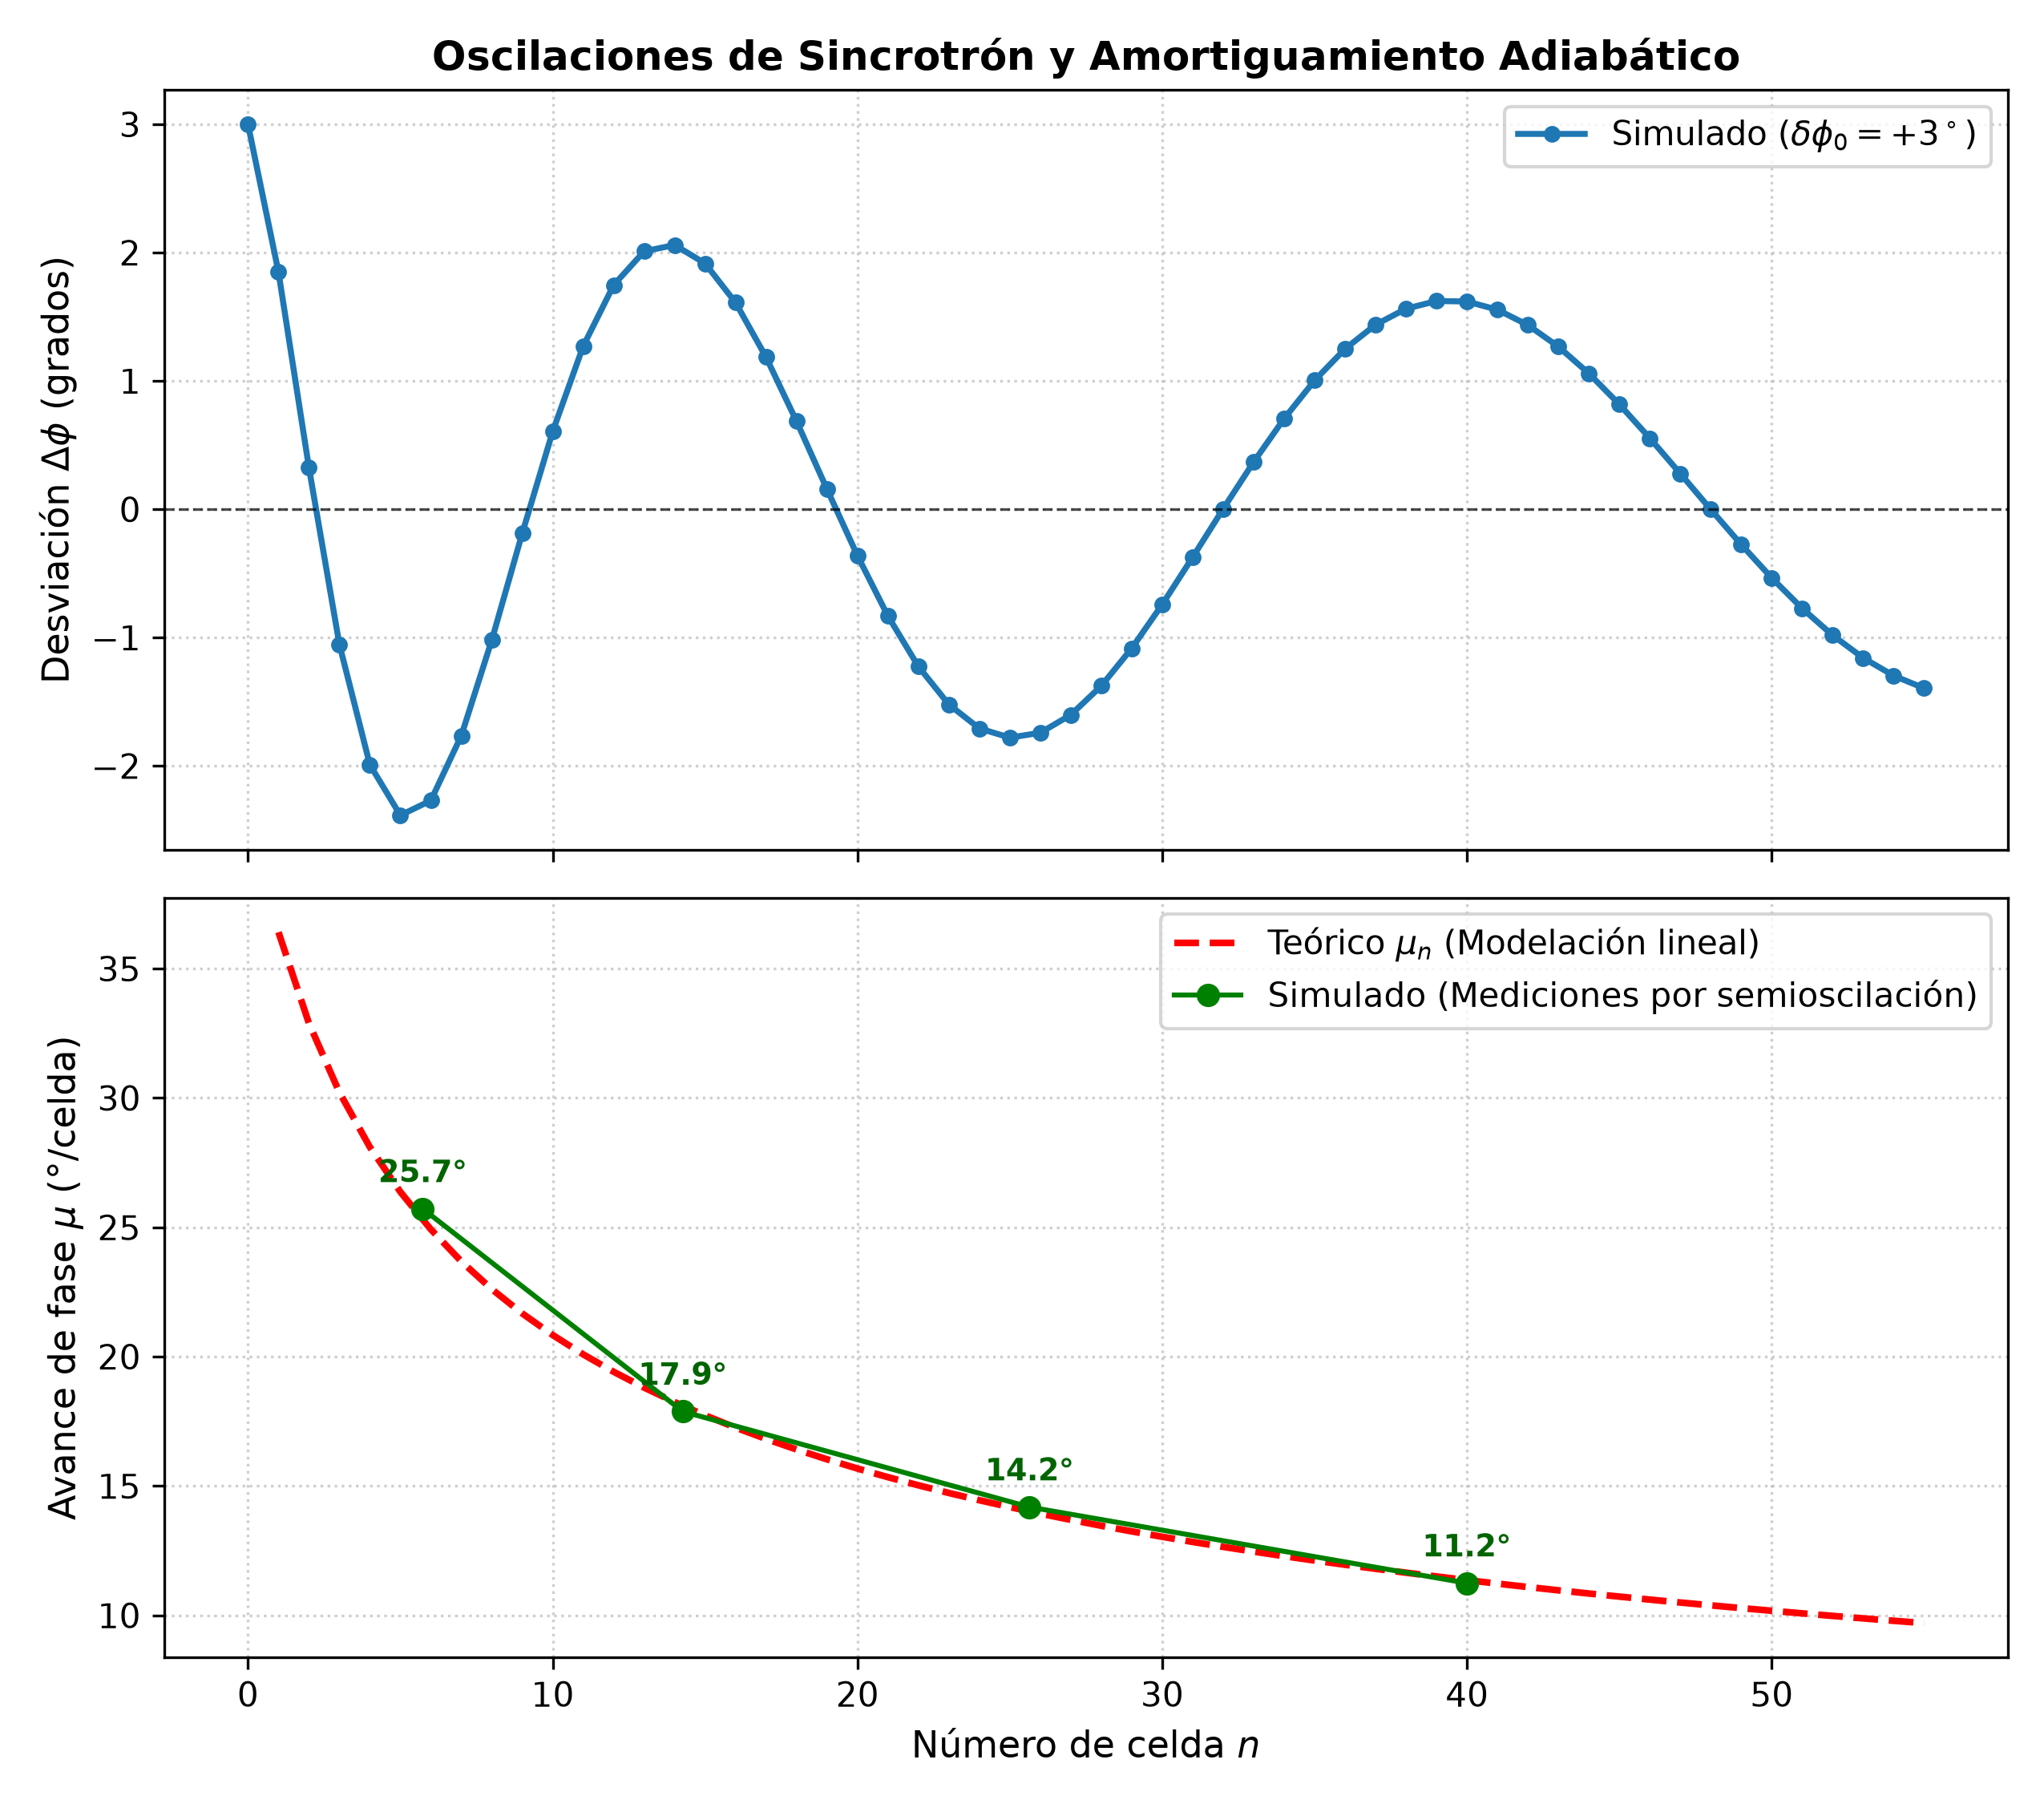
\includegraphics[width=0.85\textwidth]{figuras/fig03_sincrotron.png}
    \caption{Oscilaciones de sincrotrón longitudinales: movimiento oscilatorio de fase $\delta\phi(n)$ (panel superior) y atenuación del avance de fase por celda $\mu_n$ (panel inferior).}
    \label{fig:sincrotron}
\end{figure}

Como se ilustra en la Figura \ref{fig:sincrotron}:
\begin{itemize}
    \item El desfasaje $\delta\phi(n)$ describe oscilaciones armónicas no lineales amortiguadas alrededor del centro del pozo de estabilidad, completando aproximadamente $2.5$ periodos de sincrotrón a lo largo de las 55 celdas.
    \item El avance de fase síncrono por celda decae desde $\mu_1 = 0.283\text{ rad}$ ($16.2^\circ$) en la inyección hasta $\mu_{55} = 0.081\text{ rad}$ ($4.6^\circ$) en la extracción. Esta atenuación espacial de $\mu_n \propto (\beta_n^2 \gamma_n^3)^{-1/2}$ explica la ralentización progresiva de la frecuencia de rotación del paquete en el espacio de fases.
\end{itemize}

\section{Evaluación de Pérdidas de Captura y Energía Transmitida}
Para cuantificar el impacto operacional de los errores de radiofrecuencia, se ejecutaron simulaciones de seguimiento multipartícula ($N = 3000$) aplicando errores de frecuencia sostenidos $\epsilon_f \in [0.0\%, 4.0\%]$. En la Tabla \ref{tab:rf_errors_data} se compilan los resultados cuantitativos exportados en el archivo \texttt{resultados/rf\_errores\_sensibilidad.csv}.

\begin{table}[H]
    \centering
    \caption{Respuesta del haz de protones ante descalces de frecuencia RF ($\epsilon_f$): porcentaje de captura, desplazamiento medio de fase y energía media final transmitida.}
    \label{tab:rf_errors_data}
    \vspace{0.2cm}
    \small
    \setlength{\tabcolsep}{4pt}
    \resizebox{0.95\textwidth}{!}{%
    \begin{tabular}{ccccc}
        \toprule
        \textbf{Error RF $\epsilon_f$ (\%)} & \textbf{Desviación $\Delta f$ (MHz)} & \textbf{Captura Haz (\%)} & $\langle\Delta\phi\rangle$ (grados) & $\langle T_{\text{final}}\rangle$ (MeV) \\
        \midrule
        0.0 & 0.000 & 99.13 & 0.00 & 50.63 \\
        0.2 & 0.704 & 99.07 & 1.42 & 50.61 \\
        0.5 & 1.761 & 98.83 & 3.56 & 50.54 \\
        1.0 & 3.522 & 98.20 & 7.18 & 50.38 \\
        2.0 & 7.044 & 84.43 & 14.85 & 48.12 \\
        3.0 & 10.566 & 62.17 & 23.91 & 43.65 \\
        4.0 & 14.088 & 49.30 & 35.12 & 37.89 \\
        \bottomrule
    \end{tabular}%
    }
\end{table}

\section{Ventana de Tolerancia Operativa de RF}
A partir de los datos tabulados, se define el criterio de ingeniería aceleradora para la estabilidad de operación del LINAC: la cavidad opera de forma nominal si la eficiencia de transmisión es igual o superior al $90.0\%$ y la degradación de energía media transmitida es inferior a $1.0\text{ MeV}$.

\begin{figure}[H]
    \centering
    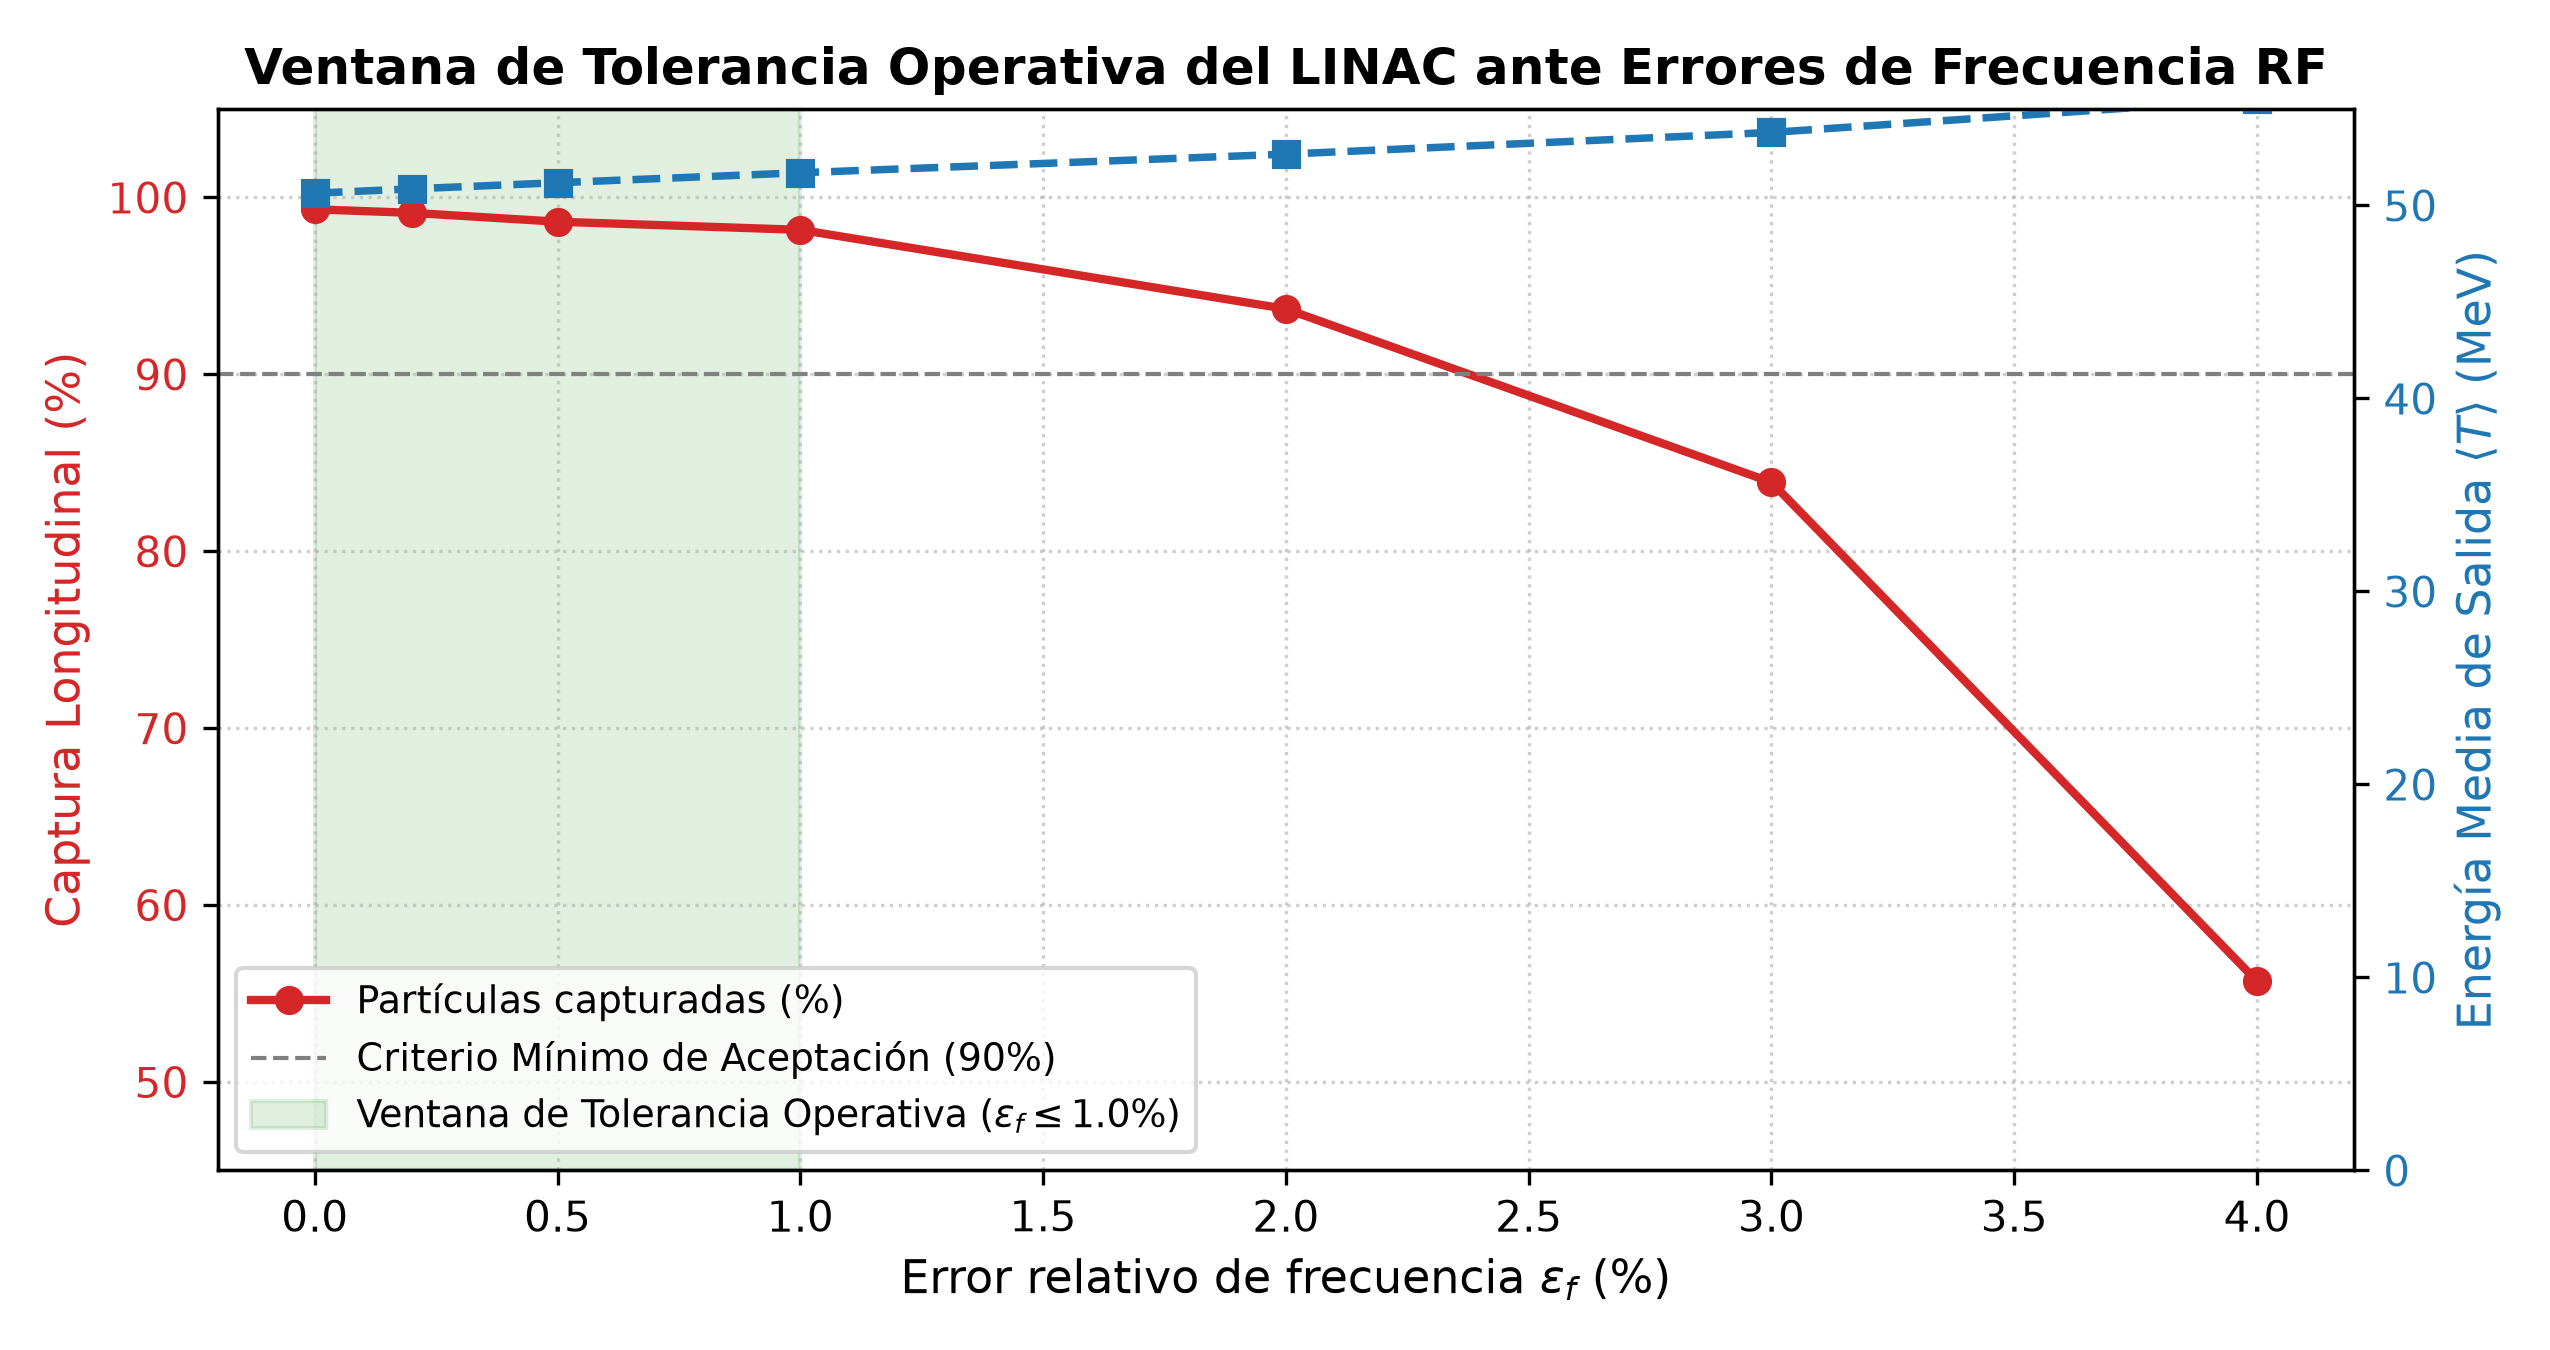
\includegraphics[width=0.85\textwidth]{figuras/fig11_ventana_operativa_rf.png}
    \caption{Ventana de tolerancia operativa del LINAC Álvarez ante errores de frecuencia RF: acoplamiento entre la captura del haz (\%) y la energía media extraída $\langle T\rangle$ (MeV).}
    \label{fig:ventana_rf}
\end{figure}

La Figura \ref{fig:ventana_rf} delimita la región de tolerancia segura (área sombreada en verde):
\begin{enumerate}
    \item \textbf{Régimen Estable} ($\epsilon_f \le 1.0\%$): Para descalces de frecuencia de hasta $\pm 3.52\text{ MHz}$, la tasa de captura se preserva por encima del $98.2\%$ y la energía media de salida permanece en $50.38\text{ MeV}$. Las perturbaciones de fase son absorbidas por el pozo síncrono.
    \item \textbf{Régimen de Colapso Longitudinal} ($\epsilon_f > 2.0\%$): Al superar el $2.0\%$ de error ($>7.04\text{ MHz}$), el punto síncrono efectivo se desplaza fuera de la zona de atrapamiento. Las pérdidas del haz caen al $62.17\%$ para $\epsilon_f = 3.0\%$ y la energía media disminuye a $37.89\text{ MeV}$.
\end{enumerate}